\subsection{Dependency Probing (RQ4)}
\label{sec:rq4}


\subsubsection{Attentions between Statements}~\\
Figure~\ref{fig:rq4-attention} shows the attention weights, at the output layer, for the last three \code{try} block statements in the code example given in Figure~\ref{fig:rq1-case}. We used the tool BertViz to make the visualization; Darker lines mean the attention weights are higher. 

Statement 7 defines an \code{InputStream} object which puts the most attention weight on itself (Figure~\ref{fig:stmt-7}). Statement 8 invokes \code{readAllBytes()} on the \code{InputStream} object; In Figure~\ref{fig:stmt-8}, we see that it indeed puts the most attention on Statement 7. In Figure~\ref{fig:stmt-9}, we see that Statement 9 attends to Statements 7 and 8 (besides itself), reflecting the data dependencies between statements. None of the three statements put much attention on any statement outside the \code{try} block. Also, note that these statements contain important APIs with respect to correctly catching the \code{IOException}. Therefore, we argure that through the attention mechanism, {\tool} is able to better understand important API calls from the context in order to recommend exceptions.
\begin{figure}
     \centering
     \begin{subfigure}[b]{0.15\textwidth}
         \centering
         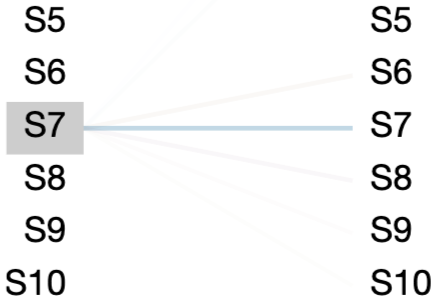
\includegraphics[width=\textwidth]{sec9-fig1.png}
         \caption{Statement 7}
         \label{fig:stmt-7}
     \end{subfigure}
     \hfill
     \begin{subfigure}[b]{0.15\textwidth}
         \centering
         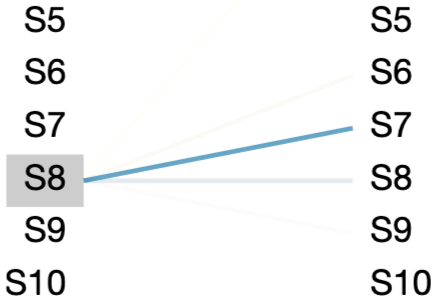
\includegraphics[width=\textwidth]{sec9-fig2.png}
         \caption{Statement 8}
         \label{fig:stmt-8}
     \end{subfigure}
     \hfill
     \begin{subfigure}[b]{0.15\textwidth}
         \centering
         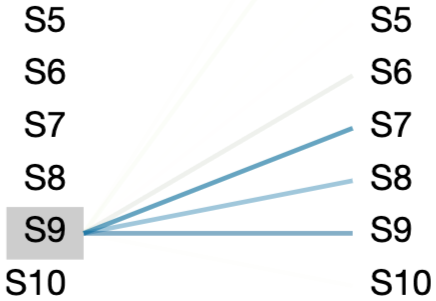
\includegraphics[width=\textwidth]{sec9-fig3.png}
         \caption{Statement 9}
         \label{fig:stmt-9}
     \end{subfigure}
        \caption{Attentions between Statements}
        \label{fig:rq4-attention}
\end{figure}


\subsubsection{Distances between Statement Embeddings}~\\
The confidence interval of the mean of cosine distances for the inside
statement group is 0.1262 to 0.1268 with 95\% confidence, and the
confidence interval for the inside-to-outside statement group is
0.7987 to 0.8001 with 95\% confidence. As seen in
Figure~\ref{fig:rq4-density}, the distribution of the cosine distances
for all the inside-to-outside statement pairs is largely to the right
of the distribution for all the inside statement pairs. That is,
{\tool} tends to {\em encode statements in a way that the statements
  in the same \code{try-catch} block are closer to each other in the
  embedding space}, leading to better grouping.
  
\begin{figure}[t]
 	\centering
 	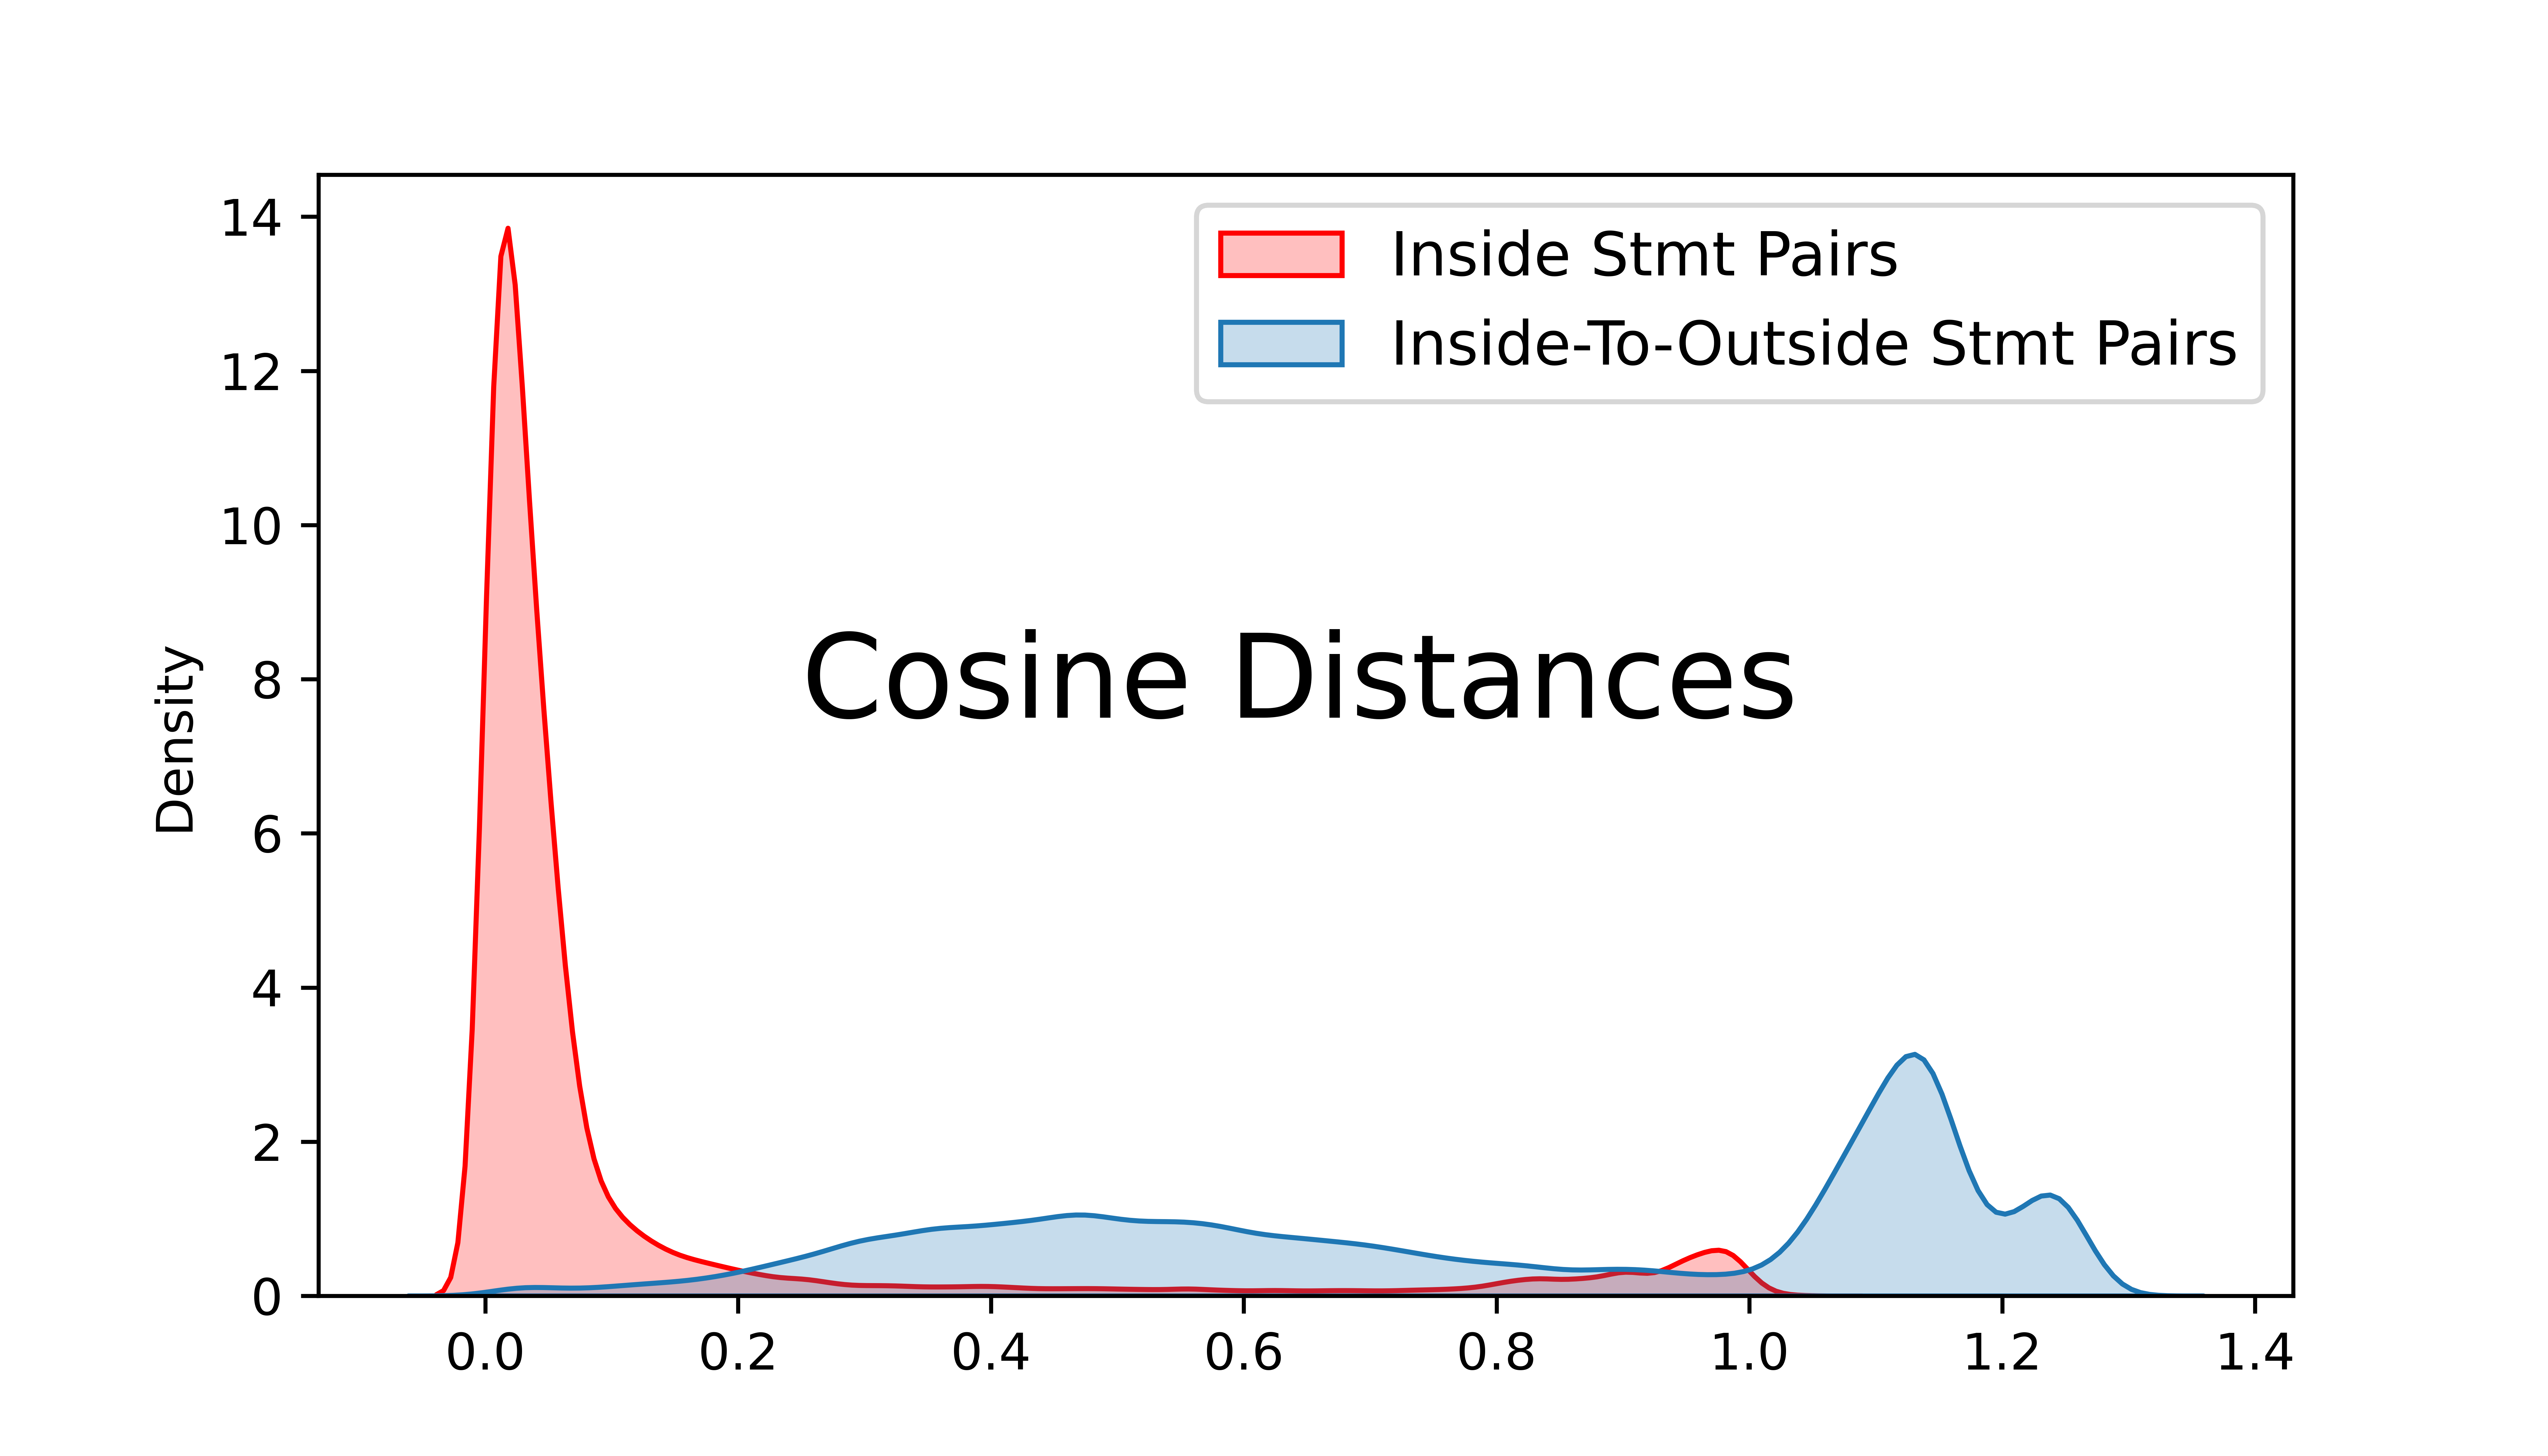
\includegraphics[width=2.8in]{rq4-density-v2.png}
        \vspace{-12pt}
 	\caption{The Distribution of Cosine Distances}
 	\label{fig:rq4-density}	
\end{figure}




